\documentclass[11pt]{amsart}
\usepackage[margin=1.15in]{geometry}
\usepackage{amssymb,mathtools,booktabs,graphicx,microtype,flafter}
\usepackage[hidelinks]{hyperref}

\newtheorem{theorem}{Theorem}[section]
\newtheorem{proposition}[theorem]{Proposition}
\newtheorem{lemma}[theorem]{Lemma}
\newtheorem{corollary}[theorem]{Corollary}
\theoremstyle{definition}
\newtheorem{definition}[theorem]{Definition}
\newtheorem{conjecture}[theorem]{Conjecture}
\newtheorem{observation}[theorem]{Numerical result}
\theoremstyle{remark}
\newtheorem{remark}[theorem]{Remark}

\newcommand{\C}{\mathbb{C}}
\newcommand{\D}{\mathbb{D}}
\newcommand{\Z}{\mathbb{Z}}
\newcommand{\Q}{\mathbb{Q}}
\newcommand{\R}{\mathbb{R}}
\newcommand{\PP}{\mathcal{P}_0}
\newcommand{\Ph}{\mathcal{P}_{1/2}}
\newcommand{\Res}{\operatorname*{Res}}
\newcommand{\resit}{\operatorname{r\acute{e}sit}}

\begin{document}

\title[Beyond the Ford-circle law]{Beyond the Ford-circle law:\\ parabolic renormalization and the shape\\ of Mandelbrot satellite bulbs}
\author{Lars Bendixen}
\date{September 2026}
\subjclass[2020]{Primary 37F46; Secondary 37F25, 37F10, 11A55}
\keywords{Mandelbrot set, satellite components, Ford circles, holomorphic index, r\'esidu it\'eratif, parabolic implosion, horn map, near-parabolic renormalization}

\begin{abstract}
To first order, the satellite component of the Mandelbrot set attached to the main cardioid at internal angle $p/q$ is a round disc of diameter proportional to $q^{-2}$; this is the Ford-circle law. We study the first correction. Expanding the multiplier of the bifurcating $q$-cycle in the bulb-scale parameter $u=q^2\varepsilon$, we prove that the first coefficient depending on $p/q$ is $\kappa(p/q)=(\iota_{p/q}-\frac12)/q$, where $\iota_{p/q}$ is the holomorphic index of the parabolic fixed point of $f^q$. We also prove that $\kappa(p/q)+\frac12$ is the index of the rotation quotient of $f^q$, and we give an exact $O(q^2)$ recursion for it. We then present numerical evidence, at up to $27$ digits, that the correction is governed by parabolic renormalization. The limit $\kappa_0=\lim\kappa(1/q)$ equals $\iota(\PP)-\frac12$, where $\PP$ is the parabolic renormalization of $z+z^2$. Along bounded $p$, the limits of $\kappa$ and of the bulb diameter are those of $\PP$ times the Inou--Shishikura phase. The entire $O(1/q)$ correction is kinematic, because the exact phase is a M\"obius function of $u$. Along continued fractions with large partial quotients the constants form a hierarchy that converges geometrically, with ratio $0.042$, to a constant $\kappa_*$ attached to the fixed point of parabolic renormalization composed with complex conjugation, which is not the Inou--Shishikura fixed point. Components differ only through the germ at their root: the period-two disc is governed by the renormalization of $-z+z^2$. The cubic family $z^3+c$ forms a second universality class. We compute three new constants to 30 digits, and no integer relation with classical constants is found.
\end{abstract}

\maketitle

\section{Introduction}\label{sec:intro}

\subsection{The Ford-circle law and its first correction}
Let $\lambda\in\D$ parametrize the main cardioid of the Mandelbrot set $M$ by the multiplier of the attracting fixed point, $c(\lambda)=\lambda/2-\lambda^2/4$. Equivalently we work with
\[
f_\lambda(z)=\lambda z+z^2 ,
\]
which is affinely conjugate to $z^2+c(\lambda)$. At each root of unity $\lambda_0=e^{2\pi i p/q}$, $\gcd(p,q)=1$, a satellite hyperbolic component $W_{p/q}$ of period $q$ is attached to the cardioid~\cite{DH}. Its size is of order $q^{-2}$~\cite{GM}. More precisely, to first order in $1/q$ it is a round disc of diameter $2|c'(\lambda_0)|q^{-2}=2\sin(\pi p/q)\,q^{-2}$~\cite{FM}. These diameters and the tangency pattern of the $W_{p/q}$ are those of the Ford circles~\cite{Ford}, which is the leading-order content of the familiar analogy between $M$ and the Farey tessellation.

This paper studies the \emph{first correction} to that law, which to our knowledge has not been investigated before. Put $\lambda=\lambda_0e^{\varepsilon}$ and let $\rho_{p/q}(\varepsilon)$ be the multiplier of the $q$-cycle of $f_\lambda$ that bifurcates from the fixed point $0$. In the bulb-scale variable $u=q^2\varepsilon$ write
\begin{equation}\label{eq:R}
R_{p/q}(u):=\rho_{p/q}(u/q^2)=\sum_{k\ge0} r_k(p/q)\,u^k .
\end{equation}
Up to the conformal change of variable $u\mapsto c(\lambda_0e^{u/q^2})$, the component $W_{p/q}$ is the set $\{|R_{p/q}(u)|<1\}$. We show that $r_0=1$ and $r_1=-1$ for every $p/q$, so that to first order $W_{p/q}$ is the disc $|u-1|<1$: this is the Ford law. The first coefficient that depends on $p/q$ is
\[
\kappa(p/q):=r_2(p/q),
\]
and it governs the leading deviation of $W_{p/q}$ from a round disc.

\subsection{Exact results}
Let $f=f_{\lambda_0}$, so that $f^q(z)=z+a\,z^{q+1}+O(z^{q+2})$ with $a\ne0$, and let $\iota_{p/q}=\Res_{z=0}dz/(z-f^q(z))$ be the holomorphic index of $0$ as a fixed point of $f^q$.

\begin{itemize}
\item \textbf{Index formula} (Theorem~\ref{thm:index}). $\rho_{p/q}(\varepsilon)=1-q^2\varepsilon+q^3(\iota_{p/q}-\frac12)\varepsilon^2+O(\varepsilon^3)$, that is, $\kappa(p/q)=(\iota_{p/q}-\frac12)/q$. In particular $\kappa(p/q)\in\Q(\zeta_q)$, and the values $\kappa(p'/q)$, $\gcd(p',q)=1$, form a single Galois orbit. The same holds for the satellites of every hyperbolic component of $z^d+c$.
\item \textbf{Normal form} (Theorem~\ref{thm:nf}, Corollary~\ref{cor:quotient}). If $N(z)=\lambda_0z(1+b_1z^q+b_2z^{2q})$ is the resonant normal form of $f$, then $q\,\iota_{p/q}=\frac{q^2-1}2+b_2/b_1^2$ and $\kappa(p/q)=\iota(\Phi_{p/q})-\frac12$, where $\Phi_{p/q}(W)=N^q(W^{1/q})^q$ is the $q$-fold rotation quotient of $f^q$. The coefficients $b_1,b_2$ come from an explicit recursion with $O(q^2)$ operations.
\item \textbf{Horn-map indices} (Theorem~\ref{thm:horn-index}). If $E(Z)=Z+a_0+\sum_{n\ge1}a_ne^{2\pi inZ}$ is an upper horn map and $\mathcal P(W)=W\exp(2\pi i\sum_na_nW^n)$ the corresponding parabolic germ, then $\iota(\mathcal P)-\frac12=a_2/(2\pi ia_1^2)$, independently of all normalizations.
\item \textbf{Kinematics} (Proposition~\ref{prop:kinematic}). If $\lambda=e^{2\pi i\alpha}=\lambda_0e^{u/q^2}$, then exactly $e^{-2\pi i/\alpha}=e^{-2\pi iq/p}e^{\tilde u/p^2}$, where $\tilde u=u/(1+\frac{u}{2\pi ipq})$ is a M\"obius function of $u$.
\end{itemize}

\subsection{Numerical results and conjectures}
The rest of the paper supports one picture. The rotation quotient $\Phi_{p/q}$ is, up to $O(q^{-2})$, a near-parabolic renormalization of $f_{p/q}$ in the sense of Inou and Shishikura~\cite{IS}, composed with the exact phase of Proposition~\ref{prop:kinematic}. The main consequences, each tested against the bulbs, are listed below. Table~\ref{tab:constants} collects the constants.
\begin{enumerate}
\item \emph{The constant $\kappa_0$} (\S\ref{sec:horn}). $\kappa(1/q)\to\kappa_0=\iota(\PP)-\frac12$, where $\PP$ is the parabolic renormalization of $z+z^2$. Bulbs certified to $q=32768$ and the horn map agree to $3\cdot10^{-28}$.
\item \emph{Bounded $p$ and the bulb size} (\S\ref{sec:renorm}). Along $q=pN+r$ the limits of $\kappa$ and of the bulb diameter are those of the family $e^{-2\pi ir/p}e^{u/p^2}\PP$. In ten classes with $p\le5$ they agree to at most $2.6\cdot10^{-8}$ for $\kappa$ and $9\cdot10^{-7}$ for the diameter.
\item \emph{Kinematics} (\S\ref{sec:kinematic}). $R_{p/q}(u)=\rho_{p,r}(\tilde u(u))+O(q^{-2})$ coefficientwise. This accounts for the universal term $-i/(2\pi pq)$ in $\kappa$ and for the whole $O(1/q)$ part of $R_{p/q}$.
\item \emph{The hierarchy} (\S\ref{sec:hierarchy}). Iterating along continued fractions with large partial quotients gives constants $\kappa_k$ that contract by the factor $0.042$ per level towards $\kappa_*$. The levels $k\le3$ are confirmed on bulbs. The fixed point differs from that of Lanford and Yampolsky~\cite{LY}, whose computations our code reproduces.
\item \emph{Component dependence} (\S\ref{sec:component}). The bounded-$p$ limits of a component depend only on the parabolic germ at its root. For the period-two disc this germ is $-z+z^2$, with its own constant $\kappa_{1/2}$.
\item \emph{Degree three} (\S\ref{sec:degree3}). For $z^3+c$ the same statements hold with the cusp germ $v+v^2+\frac13v^3$; the bulbs now have two antipodes (Proposition~\ref{prop:antipodes}).
\end{enumerate}

\begin{table}[t]
\centering\footnotesize
\begin{tabular}{@{}lllll@{}}
\toprule
constant & germ & value & bulbs & \\
\midrule
$\kappa_0$ & $z+z^2$ & $0.02382588740220057 - 0.05230465911400367\,i$ & $3\cdot10^{-28}$ & \S\ref{sec:horn} \\
$\kappa_0^{(3)}$ & $v+v^2+\frac13v^3$ & $0.1435992780952916 - 0.03031164789850254\,i$ & $1.3\cdot10^{-6}$ ($q=1024$) & \S\ref{sec:degree3} \\
$\kappa_{1/2}$ & $-z+z^2$ & $0.01840526161796478 - 0.04290372388023048\,i$ & $3\cdot10^{-10}$ & \S\ref{sec:component} \\
$\kappa_*$ & $G_*=\mathcal P(\bar G_*)$ & $0.011929183413 - 0.037455493752\,i$ & levels $\le3$ & \S\ref{sec:hierarchy} \\
$G_0$ & $e^{u}\mathcal P_0$ & $1.02641539$ & $4\cdot10^{-8}$ & \S\ref{sec:unfolding} \\
\bottomrule
\end{tabular}

\caption{The constants of this paper. The column ``bulbs'' gives the agreement between the horn-map value and the limit extracted from the bulbs; for $\kappa_0^{(3)}$ it gives the error at $q=1024$, which decays like $q^{-2}$.}\label{tab:constants}
\end{table}

We state as conjectures only what the evidence supports quantitatively: Conjectures~\ref{conj:main}, \ref{conj:unfolding}, \ref{conj:hierarchy} and~\ref{conj:root}. All numerical results are obtained either in certified ball arithmetic or by two independent computations, and they are stated with their error estimates (Appendix~\ref{app:num}).

\subsection{Related work}
The $q^{-2}$ law is due to Guckenheimer and McGehee~\cite{GM}, and the leading constant $2\sin(\pi p/q)$ was derived by Fowler and McGuinness~\cite{FM}. Parabolic implosion and horn maps go back to Douady, Lavaurs and Shishikura~\cite{Lavaurs,Sh}. Near-parabolic renormalization and its invariant class are due to Inou and Shishikura~\cite{IS}, and Lanford and Yampolsky~\cite{LY} studied the fixed point of parabolic renormalization numerically. The holomorphic index and the r\'esidu it\'eratif are classical~\cite{Milnor,Ecalle,BE}. The Ford-circle analogy is usually stated only to leading order, and we are not aware of previous work on the corrections.

\subsection{Organization}
Section~\ref{sec:index} proves the index formula, and Section~\ref{sec:nf} gives the normal form and the rotation quotient. Section~\ref{sec:horn} treats the horn map of $z+z^2$ and $\kappa_0$. Section~\ref{sec:renorm} formulates the renormalization principle and tests it at bounded $p$ and at first order in $1/q$. Sections~\ref{sec:hierarchy} and~\ref{sec:component} treat the hierarchy and the dependence on the component, and Section~\ref{sec:degree3} treats degree three. Section~\ref{sec:pslq} reports integer-relation searches, and Section~\ref{sec:discussion} lists open problems. The appendix describes the numerical methods.

\section{The index formula}\label{sec:index}

Fix $p/q$ in lowest terms, $\lambda_0=e^{2\pi ip/q}$, and write $f=f_{\lambda_0}$. Since $f$ has a single critical point, the parabolic fixed point $0$ has exactly one cycle of $q$ attracting petals, so
\begin{equation}\label{eq:fq}
f^q(z)=z+a\,z^{q+1}+O(z^{q+2}),\qquad a=a(p/q)\neq0 .
\end{equation}
The holomorphic index~\cite[\S12]{Milnor} of $0$ as a fixed point of $f^q$ is
\[
\iota_{p/q}:=\frac1{2\pi i}\oint\frac{dz}{z-f^q(z)}=\Res_{z=0}\frac{dz}{z-f^q(z)},
\]
and its r\'esidu it\'eratif~\cite{Ecalle,BE} is $\resit=\frac{q+1}{2}-\iota_{p/q}$.

\begin{theorem}[Index formula]\label{thm:index}
The multiplier $\rho_{p/q}(\varepsilon)$ of the $q$-cycle of $f_{\lambda_0e^\varepsilon}$ that bifurcates from $0$ is holomorphic near $\varepsilon=0$, and
\[
\rho_{p/q}(\varepsilon)=1-q^2\varepsilon+q^3\Bigl(\iota_{p/q}-\frac12\Bigr)\varepsilon^2+O(\varepsilon^3).
\]
Equivalently, in \eqref{eq:R}, $r_0=1$, $r_1=-1$ and $\kappa(p/q)=(\iota_{p/q}-\frac12)/q$.
\end{theorem}

\begin{proof}
Choose a disc $D$ around $0$ on whose boundary $z\ne f^q(z)$ and which contains no other fixed point of $f^q$. By \eqref{eq:fq} and Rouch\'e's theorem, for $|\varepsilon|$ small the map $f_\lambda^q$, $\lambda=\lambda_0e^\varepsilon$, has exactly $q+1$ fixed points in $D$, counted with multiplicity. One of them is $0$, with multiplier $\lambda^q=e^{q\varepsilon}\neq1$, so it is simple. For each proper divisor $d$ of $q$ the map $f^d$ has multiplier $\lambda_0^d\ne1$ at $0$, so $f_\lambda^d$ has no fixed point in $D$ other than $0$. The remaining $q$ points therefore have exact period $q$ and form a single cycle; call its multiplier $\rho(\varepsilon)$. The cycle, as an unordered set, depends holomorphically on $\lambda$, hence so does $\rho$, which is a symmetric function of the cycle points. The function $\rho$ is not identically $1$, since the cycle is attracting on the satellite, so for $\varepsilon\ne0$ small all $q+1$ fixed points are simple. Summing their indices $1/(1-m)$ gives
\begin{equation}\label{eq:sum}
\frac1{1-e^{q\varepsilon}}+\frac q{1-\rho(\varepsilon)}=\frac1{2\pi i}\oint_{\partial D}\frac{dz}{z-f_\lambda^q(z)}\xrightarrow[\varepsilon\to0]{}\iota_{p/q},
\end{equation}
because the integrand converges uniformly on $\partial D$. The first term equals $-1/(q\varepsilon)+\frac12+O(\varepsilon)$ and is unbounded. Hence $\rho(0)=1$. Writing $1-\rho=A\varepsilon^m(1+O(\varepsilon))$ with $A\ne0$, boundedness of the sum forces $m=1$ and $A=q^2$. With $\rho=1-q^2\varepsilon+C\varepsilon^2+O(\varepsilon^3)$ we get $q/(1-\rho)=1/(q\varepsilon)+C/q^3+O(\varepsilon)$, and \eqref{eq:sum} yields $\frac12+C/q^3=\iota_{p/q}$.
\end{proof}

\begin{remark}[Other components]\label{rem:general}
The proof uses only that the parabolic point has multiplicity $q+1$. It therefore applies verbatim to the satellites of any hyperbolic component of $z^d+c$, whose parabolic cycles have a single cycle of petals, with $\lambda$ the multiplier of the attracting cycle of that component and $f^q$ replaced by the first return map. We checked numerically, for the period-two disc and for $z^3+c$, that $r_2=(\iota-\frac12)/q$ holds to $10^{-7}$ at $p/q=2/7$ and $3/11$.
\end{remark}

\begin{remark}[Exact values]\label{rem:exact}
Since $f^q$ has coefficients in $\Z[\lambda_0]$, the index is a rational function of $\lambda_0$ with rational coefficients. Hence $\iota_{p/q}\in\Q(\zeta_q)$ and $\iota_{p'/q}=\sigma(\iota_{p/q})$ for the automorphism $\sigma:\zeta_q\mapsto\zeta_q^{p'\bar p}$, where $p\bar p\equiv1\pmod q$. For example $\iota_{1/2}=\frac18$, $\iota_{1/3}=\frac{100-8\sqrt3\,i}{441}$ and $\iota_{1/4}=\frac{1447-365\,i}{4624}$, so that $\kappa(1/2)=-\frac3{16}$ and $\kappa(1/3)=\frac{-241-16\sqrt3\,i}{2646}$.
\end{remark}

\begin{definition}\label{def:G}
Let $c_{\rm root}=c(\lambda_0)$, and let $c_{\rm ant}\in\partial W_{p/q}$ be the boundary point at which the $q$-cycle has multiplier $-1$. It is unique because in degree two the multiplier map $W_{p/q}\to\D$ is a conformal isomorphism. Set
\[
d(p/q)=|c_{\rm ant}-c_{\rm root}|,\qquad G(p/q)=\frac{d(p/q)}{2|c'(\lambda_0)|\,q^{-2}} .
\]
Since $c(\lambda_0e^{u/q^2})-c(\lambda_0)=c'(\lambda_0)\lambda_0u/q^2+O(q^{-4})$, we have $G(p/q)=\tfrac12|u_a|+O(q^{-2})$, where $R_{p/q}(u_a)=-1$. To first order $u_a=2$ and $G=1$, and the deviation of $G$ from $1$ is governed at leading order by $\kappa$.
\end{definition}

\section{Normal forms and the rotation quotient}\label{sec:nf}

\begin{theorem}[Normal form]\label{thm:nf}
There is a unique formal conjugacy $H(z)=z+\sum_{k\ge2}H_kz^k$ with $H_{q+1}=H_{2q+1}=0$ such that $f\circ H=H\circ N$ up to order $2q+1$, where
\[
N(z)=\lambda_0z\bigl(1+b_1z^q+b_2z^{2q}\bigr).
\]
Put $\beta_i=\lambda_0b_i$ and let $(H^2)_k$ denote the coefficient of $z^k$ in $H(z)^2$. The coefficients are determined by the recursion
\begin{equation}\label{eq:rec}
H_k(\lambda_0-\lambda_0^k)=[k>q+1]\,(k-q)\lambda_0^{k-q-1}\beta_1H_{k-q}-(H^2)_k\quad(2\le k\le 2q,\ k\ne q+1),
\end{equation}
together with $\beta_1=(H^2)_{q+1}$ and $\beta_2=(H^2)_{2q+1}$. Moreover
\[
a(p/q)=q\,b_1,\qquad q\,\iota_{p/q}=\frac{q^2-1}{2}+\frac{b_2}{b_1^2},\qquad
\kappa(p/q)=\frac12-\frac1{2q}-\frac1{2q^2}+\frac{b_2}{(qb_1)^2}.
\]
\end{theorem}

\begin{proof}
Comparing coefficients of $z^k$ in $\lambda_0H+H^2=\sum_mH_m N^m$ gives \eqref{eq:rec}. Here we use that $[N^m]_k$ is nonzero only for $k\in\{m,\,m+q,\,m+2q\}$, with values $\lambda_0^m$ and $m\lambda_0^{m-1}\beta_1$ in the first two cases. The factor $\lambda_0-\lambda_0^k$ vanishes exactly when $k\equiv1\pmod q$. At $k=q+1$ and $k=2q+1$ the equation fixes $\beta_1$ and $\beta_2$ and leaves $H_{q+1}$ and $H_{2q+1}$ free; we set them to zero. For the second part, write $N^j(z)=\lambda_0^jz(1+A_jz^q+B_jz^{2q}+\dots)$. Using $\lambda_0^q=1$ and $(N^j)^q=z^q(1+qA_jz^q+\dots)$,
\[
A_{j+1}=A_j+b_1,\qquad B_{j+1}=B_j+(q+1)b_1A_j+b_2,
\]
so $A_q=qb_1$ and $B_q=\frac{(q+1)q(q-1)}2b_1^2+qb_2$. The coefficient $a$ and the index are invariant under formal conjugacy tangent to the identity, and for $z+Az^{q+1}+Bz^{2q+1}$ the index is $B/A^2$. This gives the formulas for $a$ and $\iota$, and the formula for $\kappa$ follows from Theorem~\ref{thm:index}.
\end{proof}

\begin{corollary}[$\kappa$ is an index]\label{cor:quotient}
Since $N$ commutes with $z\mapsto\lambda_0z$, the rotation quotient $\Phi_{p/q}(W):=N^q(W^{1/q})^q=W+q^2b_1W^2+\dots$ is a well-defined germ, and
\[
\kappa(p/q)=\iota(\Phi_{p/q})-\tfrac12=\tfrac12-\resit(\Phi_{p/q}).
\]
\end{corollary}

\begin{proof}
From $N^q(z)=z(1+A_qz^q+B_qz^{2q}+\dots)$ we get $\Phi(W)=W(1+A_qW+B_qW^2)^q+\dots$. Hence $\Phi=W+AW^2+BW^3+\dots$ with $A=qA_q=q^2b_1$ and $B=qB_q+\binom q2A_q^2$. Then $\iota(\Phi)=B/A^2=1-\frac1{2q}-\frac1{2q^2}+\frac{b_2}{(qb_1)^2}$, which is $\kappa+\frac12$ by Theorem~\ref{thm:nf}.
\end{proof}

\begin{remark}[Computation]\label{rem:computation}
The recursion \eqref{eq:rec} costs $O(q^2)$ arithmetic operations. It is numerically stable: at $q=128$ and $q=301$ the computed $\kappa(1/q)$ does not change in more than twenty digits when the working precision is raised from $60$ to over $300$ digits, and for generic $p$ with $q$ up to $6.4\cdot10^4$ two runs at $128$ and $192$ bits agree to $10^{-34}$. By contrast, composing $f$ symbolically $q$ times costs $O(q^3)$ and loses about $q$ decimal digits to cancellation at $p=1$, where $|a(1/q)|\approx e^{2.3q}$. With a blocked online convolution the recursion runs in ball arithmetic~\cite{Arb}, which certifies $\kappa(1/q)$ for $q\le32768$ (Appendix~\ref{app:num}).
\end{remark}

\section{The horn map of $z+z^2$ and the constant $\kappa_0$}\label{sec:horn}

\subsection{The limit along $1/q$}
Table~\ref{tab:kappa1q} and Figure~\ref{fig:conv} show $\kappa(1/q)$ for $q$ up to $32768$.

\begin{table}[t]
\centering\small
\begin{tabular}{@{}rll@{}}
\toprule
$q$ & $\kappa(1/q)$ & $|\kappa(1/q)+\tfrac{i}{2\pi q}-\kappa_0|$ \\
\midrule
64 & $0.02385454027565757 - 0.05408067667475267\,i$ & $7.1\cdot10^{-4}$ \\
256 & $0.02383094323212187 - 0.05288194473715776\,i$ & $4.5\cdot10^{-5}$ \\
1024 & $0.02382625451962614 - 0.05245731336604759\,i$ & $2.8\cdot10^{-6}$ \\
4096 & $0.02382591114406885 - 0.05234334224894280\,i$ & $1.7\cdot10^{-7}$ \\
8192 & $0.02382589337085374 - 0.05232404394907701\,i$ & $4.4\cdot10^{-8}$ \\
16384 & $0.02382588889851146 - 0.05231436234675194\,i$ & $1.1\cdot10^{-8}$ \\
32768 & $0.02382588777679670 - 0.05230951343396723\,i$ & $2.7\cdot10^{-9}$ \\
\midrule
fit, $q\to\infty$ & $0.02382588740220057 - 0.05230465911400367\,i$ & \\
horn map, Num.~res.~\ref{obs:identity} & $0.02382588740220057 - 0.05230465911400367\,i$ & \\
\bottomrule
\end{tabular}

\caption{$\kappa(1/q)$ from the normal-form recursion (first sixteen digits shown). The corrected error decays like $q^{-2}$. Values for $q\ge1024$ are certified in ball arithmetic (radius $\le5.4\cdot10^{-44}$). The fit uses the thirteen values $256\le q\le 32768$ with eleven terms in $1/q$ (residual $3.6\cdot10^{-29}$). The last row is the horn-map value of Numerical result~\ref{obs:identity}.}\label{tab:kappa1q}
\end{table}

\begin{observation}\label{obs:limit}
Least-squares fits $\kappa(1/q)=\sum_{j\le J}c_jq^{-j}$ over $q\ge q_{\min}$ are stable under changes of $(q_{\min},J)$. The best overdetermined fit, $(q_{\min},J)=(256,10)$ on thirteen values with residual $3.6\cdot10^{-29}$, gives
\[
c_0=0.023825887402200569000729189645\ldots-0.052304659114003666316522486208\ldots\,i ,
\]
the first-order coefficient $c_1=-i/(2\pi)$ to within $2\cdot10^{-23}$, and $c_2=0.402776138694+2.902726170410\,i$. The ratios $|c_{j+1}/c_j|$ stay near $7$, consistent with an expansion that converges for $q\gtrsim7$.
\end{observation}

\begin{figure}[t]
\centering
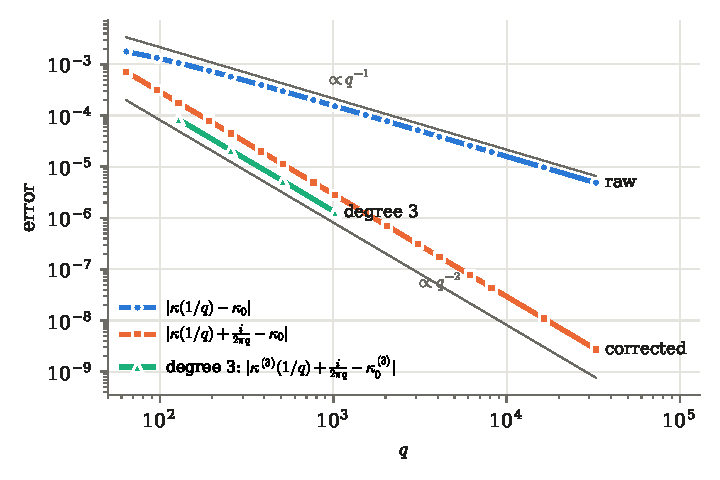
\includegraphics[width=0.78\textwidth]{figures/convergence.pdf}
\caption{Convergence of $\kappa(1/q)$ to $\kappa_0$ in degree two and of $\kappa_3(1/q)$ to $\kappa_0^{(3)}$ in degree three (Section~\ref{sec:degree3}). The raw error decays like $q^{-1}$; after the universal correction $-i/(2\pi q)$ it decays like $q^{-2}$.}\label{fig:conv}
\end{figure}

\subsection{Fatou coordinates and the horn map}
We recall the objects of parabolic implosion~\cite{Lavaurs,Sh,IS,LY} in the form in which we compute them. In the coordinate $w=-1/z$ the map $f_0(z)=z+z^2$ becomes
\[
F(w)=\frac{w^2}{w-1}=w+1+\frac1{w-1}.
\]

\begin{lemma}[Formal Fatou coordinate]\label{lem:fatou}
There is a unique formal series $\Phi(w)=w-\log w+\sum_{k\ge1}c_kw^{-k}$ with $\Phi\circ F=\Phi+1$. Its coefficients are rational,
\[c_1,c_2,\ldots=\tfrac12,\tfrac13,\tfrac{13}{36},\tfrac{113}{240},\tfrac{1187}{1800},\tfrac{877}{945},\ldots,\]
and with $u=1/w$ they satisfy the triangular system
\[
\sum_{k\ge1}c_k\bigl[(u-u^2)^k-u^k\bigr]=-\sum_{m\ge2}\Bigl(1-\frac1m\Bigr)u^m .
\]
\end{lemma}

\begin{proof}
With $u=1/w$ we have $1/F=u-u^2$, $F-w-1=u/(1-u)$ and $\log F-\log w=-\log(1-u)$. Substituting gives the displayed identity. The coefficient of $u^m$ contains $c_{m-1}$ with the factor $-(m-1)$ and otherwise only $c_k$ with $k<m-1$. The coefficient of $\log w$ is fixed by the term of order $u$; it equals the r\'esidu it\'eratif $1$ of $f_0$.
\end{proof}

Let $\Phi_{\rm att}(w)=\lim_n\bigl(\Phi(F^n(w))-n\bigr)$ on the attracting petal, with the principal logarithm, and let $\Psi_{\rm rep}(Z)=\lim_nF^n\bigl(\Phi^{-1}(Z-n)\bigr)$ be the repelling Fatou parametrization, with the branch $\arg w\in(0,2\pi)$. The upper horn map $E=\Phi_{\rm att}\circ\Psi_{\rm rep}$ commutes with $Z\mapsto Z+1$ and, for $\operatorname{Im}Z$ large, has an expansion
\[
E(Z)=Z+a_0+\sum_{n\ge1}a_ne^{2\pi inZ}.
\]
Replacing $\Phi_{\rm att}$ or $\Psi_{\rm rep}$ by a translate changes $a_0$, or conjugates $E$ by $Z\mapsto Z+c$, which sends $a_n\mapsto a_ne^{2\pi inc}$. In $W=e^{2\pi iZ}$ the horn map is the germ $W\mapsto e^{2\pi ia_0}\PP(W)$, where
\[
\PP(W):=W\exp\Bigl(2\pi i\sum_{n\ge1}a_nW^n\Bigr)
\]
is the parabolic renormalization of $f_0$, normalized to multiplier one~\cite{IS,LY}. More generally we write $\mathcal P(g)$ for the germ obtained in the same way from a parabolic germ $g$.

\begin{theorem}\label{thm:horn-index}
$\displaystyle\iota(\PP)=\frac12+\frac{a_2}{2\pi i\,a_1^2}$, and this quantity does not depend on the normalizations of the Fatou coordinates. The same formula holds for $\mathcal P(g)$.
\end{theorem}

\begin{proof}
$\PP(W)=W+AW^2+BW^3+\dots$ with $A=2\pi ia_1$ and $B=2\pi ia_2+\frac12(2\pi ia_1)^2$, and $\iota=B/A^2$. Under $a_n\mapsto a_ne^{2\pi inc}$ the ratio $a_2/a_1^2$ is unchanged, and $a_0$ does not enter.
\end{proof}

\begin{observation}\label{obs:identity}
Computing $E$ on the line $\operatorname{Im}Z=\frac14$ at 60 and at 80 digits (Appendix~\ref{app:num}) gives $a_0=0$ to working precision and
\begin{align*}
\operatorname{Re}a_1&=-0.05895043056440687000807026251551,\\
\operatorname{Im}a_1&=\phantom{-}0.010009865898273724511535250164253,\\
\operatorname{Re}a_2&=\phantom{-}0.0012858196663089284889517464706577,\\
\operatorname{Im}a_2&=\phantom{-}0.00011738770718282661923962731179377,
\end{align*}
with $|a_n|$ decreasing by a factor of about $55$ per step. Hence
\begin{align*}
\operatorname{Re}\bigl(\iota(\PP)-\tfrac12\bigr)&=\phantom{-}0.023825887402200569000729189645402,\\
\operatorname{Im}\bigl(\iota(\PP)-\tfrac12\bigr)&=-0.052304659114003666316522486207571.
\end{align*}
The two precision settings agree in all digits shown. This value coincides with $c_0$ of Numerical result~\ref{obs:limit} to $3.1\cdot10^{-28}$; other stable fits differ from it by at most $5\cdot10^{-25}$. We therefore claim agreement to at least $24$ digits, and to $27$ on the best fit.
\end{observation}

\begin{conjecture}\label{conj:main}
The limit $\kappa_0=\lim_{q\to\infty}\kappa(1/q)$ exists and equals $\iota(\PP)-\frac12=\frac{a_2}{2\pi ia_1^2}$. Moreover $\kappa(1/q)=\kappa_0-\frac{i}{2\pi q}+O(q^{-2})$.
\end{conjecture}

\section{The renormalization principle}\label{sec:renorm}

\subsection{Heuristic}
For $\alpha$ near $0$, the near-parabolic renormalization $\mathcal R$ of Inou and Shishikura~\cite{IS} assigns to $f_\alpha(z)=e^{2\pi i\alpha}z+z^2$ a germ $\mathcal Rf_\alpha$ at $0$ with multiplier $e^{-2\pi i/\alpha}$. By parabolic implosion~\cite{Lavaurs,Sh}, as $\alpha\to0$ with $-1/\alpha\to\sigma\bmod\Z$, the germ $\mathcal Rf_\alpha$ tends to $e^{2\pi i\sigma}$ times the horn germ. For $\alpha=1/q$ the phase is $0$, and $\mathcal Rf_{1/q}$ is a parabolic germ with multiplier one. The rotation quotient $\Phi_{1/q}$ of Corollary~\ref{cor:quotient} is also a parabolic germ with multiplier one, obtained from $f^q$ by passing to the quotient by the $q$-fold rotation. If $\Phi_{1/q}$ and $\mathcal Rf_{1/q}$ are conformally conjugate, Corollary~\ref{cor:quotient} and continuity of $\mathcal R$ give Conjecture~\ref{conj:main}. The same reasoning applies to the whole unfolding, and the phase can be computed exactly.

\begin{proposition}[Kinematics]\label{prop:kinematic}
Let $\lambda=e^{2\pi i\alpha}=\lambda_0e^{u/q^2}$ with $\lambda_0=e^{2\pi ip/q}$. Then $e^{-2\pi i/\alpha}=\mu\,e^{\tilde u/p^2}$, where $\mu=e^{-2\pi iq/p}$ and
\[
\tilde u=\frac{u}{1+u/(2\pi i\,pq)}=u+\frac{i\,u^2}{2\pi pq}+O\Bigl(\frac{u^3}{q^2}\Bigr).
\]
\end{proposition}

\begin{proof}
$\alpha=(2\pi ipq+u)/(2\pi iq^2)$, so $-1/\alpha+q/p=qu/\bigl(p(2\pi ipq+u)\bigr)$, and $2\pi i p^2$ times this is $\tilde u$.
\end{proof}

Fix $p\ge1$ and $r$ with $\gcd(p,r)=1$, and let $q=pN+r$. Then $\mu=e^{-2\pi ir/p}$ does not depend on $N$. Let $\rho_{p,r}(u)$ be the multiplier of the $p$-cycle of
\[
M_u(W)=\mu\,e^{u/p^2}\,\PP(W)
\]
that bifurcates from $W=0$, and write $\rho_{p,r}(u)=1-u+\kappa_{p,r}u^2+\rho_3u^3+\dots$.

\begin{conjecture}[Renormalization principle]\label{conj:unfolding}
For fixed $(p,r)$ and $q=pN+r\to\infty$,
\[
R_{p/q}(u)=\rho_{p,r}\bigl(\tilde u(u)\bigr)+O(q^{-2})
\]
coefficientwise, and locally uniformly in $u$ on the domain of $\rho_{p,r}$.
\end{conjecture}

Comparing coefficients gives the following consequences.

\begin{corollary}\label{cor:kinematic}
Under Conjecture~\ref{conj:unfolding},
\begin{equation}\label{eq:kinematic}
\kappa(p/q)=\kappa_{p,r}-\frac{i}{2\pi pq}+O(q^{-2}),\qquad r_3(p/q)=\rho_3+\frac{i\,\kappa_{p,r}}{\pi pq}+O(q^{-2}),
\end{equation}
where, by Corollary~\ref{cor:quotient} applied to $\mu\PP$,
\begin{equation}\label{eq:boundedp}
\kappa_{p,r}=\frac{\iota\bigl((\mu\PP)^p\bigr)-\frac12}{p}.
\end{equation}
Moreover $G(p/q)\to\frac12|u_a|$, where $\rho_{p,r}(u_a)=-1$.
\end{corollary}

In particular the first-order term $-i/(2\pi pq)$ involves no property of the germ, which explains why it is the same in degree three (Section~\ref{sec:degree3}). We now test the three parts of Conjecture~\ref{conj:unfolding}: the limits of $\kappa$, the whole unfolding, and the first-order correction.

\subsection{Bounded $p$}\label{sec:boundedp}
Table~\ref{tab:boundedp} compares \eqref{eq:boundedp} with bulb data for all nine classes with $2\le p\le5$. The bulb values are normal-form values of $\kappa(p/q)$ for $64\le N\le1024$, extrapolated in $1/q$. All nine agree to between $6\cdot10^{-9}$ and $2.6\cdot10^{-8}$, within the extrapolation uncertainty of about $10^{-7}$. The opposite phase convention, $\mu=e^{+2\pi ir/p}$, exchanges the classes $r$ and $p-r$ and fails. Figure~\ref{fig:cloud} places these limits within the set of all $\kappa(p/q)$ at a fixed $q$.

\begin{table}[t]
\centering\footnotesize
\begin{tabular}{@{}cclll@{}}
\toprule
$p$ & $r$ & horn-map prediction $(\iota((\mu\mathcal P_0)^p)-\frac12)/p$ & bulbs, extrapolated & $|\Delta|$ \\
\midrule
2 & 1 & $0.049693182903 - 0.023894096844\,i$ & $0.049693177608 - 0.023894071809\,i$ & $2.6\cdot10^{-8}$ \\
3 & 1 & $0.054529447219 - 0.0050171894089\,i$ & $0.054529443083 - 0.0050171743067\,i$ & $1.6\cdot10^{-8}$ \\
3 & 2 & $0.055036036944 - 0.023467983453\,i$ & $0.055036033035 - 0.023467969651\,i$ & $1.4\cdot10^{-8}$ \\
4 & 1 & $0.053737282786 + 0.0074895906470\,i$ & $0.053737279652 + 0.0074896009583\,i$ & $1.1\cdot10^{-8}$ \\
4 & 3 & $0.054739672309 - 0.026348641547\,i$ & $0.054739669177 - 0.026348633046\,i$ & $9.1\cdot10^{-9}$ \\
5 & 1 & $0.051130771685 + 0.015984969447\,i$ & $0.051130769387 + 0.015984976959\,i$ & $7.9\cdot10^{-9}$ \\
5 & 2 & $0.059925460063 - 0.010450443803\,i$ & $0.059925457760 - 0.010450436333\,i$ & $7.8\cdot10^{-9}$ \\
5 & 3 & $0.060335706660 - 0.0045365352268\,i$ & $0.060335704038 - 0.0045365278901\,i$ & $7.8\cdot10^{-9}$ \\
5 & 4 & $0.052624850350 - 0.029174853238\,i$ & $0.052624847638 - 0.029174847754\,i$ & $6.1\cdot10^{-9}$ \\
\bottomrule
\end{tabular}

\caption{Bounded-$p$ limits of $\kappa$ (degree two): the prediction \eqref{eq:boundedp} against the bulb values extrapolated from $q=pN+r$, $64\le N\le1024$.}\label{tab:boundedp}
\end{table}

\begin{figure}[t]
\centering
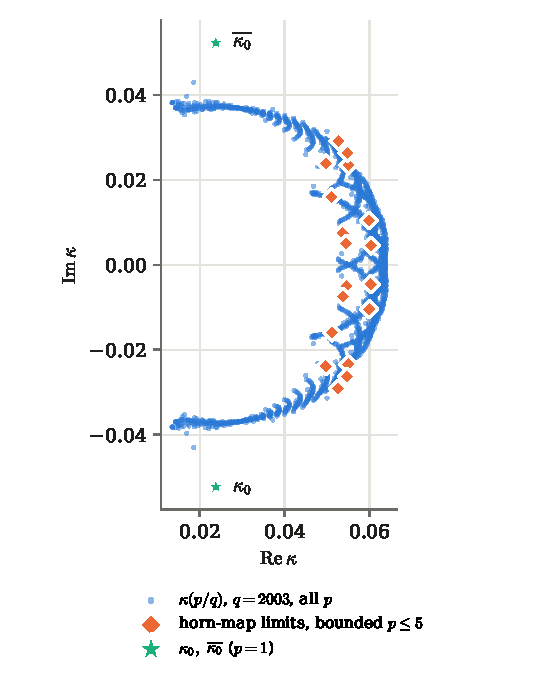
\includegraphics[width=0.52\textwidth]{figures/kappa_cloud.pdf}
\caption{All $\kappa(p/q)$ for $q=2003$ (values for $p>q/2$ from the symmetry $\kappa(1-p/q)=\overline{\kappa(p/q)}$), the limits \eqref{eq:boundedp} for $p\le5$, and $\kappa_0,\overline{\kappa_0}$. The $p=1$ bulbs are the extreme points of the arithmetic cloud.}\label{fig:cloud}
\end{figure}

\subsection{The unfolding and the bulb size}\label{sec:unfolding}
For $p=1$ the Taylor coefficients of $\rho_{1,1}$ agree with those of $R_{1/1025}$ through order eight up to the finite-$q$ shift; for instance $r_3=-3.78\cdot10^{-4}-9.80\cdot10^{-4}i$ against $-3.62\cdot10^{-4}-9.72\cdot10^{-4}i$, and $r_8=3.14\cdot10^{-9}-4.56\cdot10^{-9}i$ against $3.13\cdot10^{-9}-4.50\cdot10^{-9}i$. Since $r_3$ depends on the unfolding and not only on the germ, this checks that $u$ enters as the Lavaurs phase. The shift $r_3-\rho_3=1.6\cdot10^{-5}+0.8\cdot10^{-5}i$ is the one predicted by \eqref{eq:kinematic}, namely $1.62\cdot10^{-5}+0.74\cdot10^{-5}i$. Table~\ref{tab:G} compares the predicted bulb sizes with the bulbs for all ten classes with $p\le5$. The largest discrepancy is $9\cdot10^{-7}$. For $p=1$ this gives
\[
\lim_{q\to\infty}q^3d(1/q)=2\pi G_0,\qquad G_0=1.02641539\ldots,
\]
so the $1/q$-bulbs, which accumulate at the cusp $c=\frac14$, have diameters $2\pi G_0q^{-3}(1+O(q^{-1}))$.

\begin{table}[t]
\centering\small
\begin{tabular}{@{}ccllll@{}}
\toprule
$p$ & $r$ & $G$ at $q=512p+r$ & $G$ at $q=2048p+r$ & extrapolated & horn map \\
\midrule
1 & 1 & 1.02634395 & 1.02639633 & 1.02641535 & 1.02641539 \\
2 & 1 & 1.11142282 & 1.11143038 & 1.11143322 & 1.11143318 \\
3 & 1 & 1.12836657 & 1.12836757 & 1.12836781 & 1.12836776 \\
3 & 2 & 1.12537076 & 1.12537450 & 1.12537590 & 1.12537582 \\
4 & 1 & 1.12357397 & 1.12357381 & 1.12357368 & 1.12357348 \\
4 & 3 & 1.12156857 & 1.12157111 & 1.12157204 & 1.12157195 \\
5 & 1 & 1.11300416 & 1.11300362 & 1.11300313 & 1.11300337 \\
5 & 2 & 1.14414695 & 1.14414738 & 1.14414703 & 1.14414795 \\
5 & 3 & 1.14644523 & 1.14644563 & 1.14644539 & 1.14644595 \\
5 & 4 & 1.11312789 & 1.11312962 & 1.11312984 & 1.11313044 \\
\bottomrule
\end{tabular}

\caption{Bulb size $G$ (Definition~\ref{def:G}) along $q=pN+r$, extrapolated from $N=512,1024,2048$, against the prediction of Corollary~\ref{cor:kinematic}. The first row gives $G_0=\lim G(1/q)$.}\label{tab:G}
\end{table}

\subsection{The first-order correction}\label{sec:kinematic}
The first identity in \eqref{eq:kinematic} is the coefficient $c_1=-i/(2\pi)$ of Numerical result~\ref{obs:limit}. For $2\le p\le5$ the fitted coefficients satisfy $c_1(p)\cdot2\pi p/(-i)=1.0008,1.0011,1.0014,1.0016$, which is within the uncertainty of the fits. A sharper test uses all Taylor coefficients at once.

\begin{observation}\label{obs:kinematic}
Let $r_k(p/q)$ be the Taylor coefficients of the bulb and $\rho_k$ those of $M_u$, both computed by Cauchy integrals on $|u|=1.5$. For $2\le k\le8$, for $(p,r)=(1,1)$, $(2,1)$, $(3,1)$ and $(3,2)$, and for $N=64,128,\dots,1024$, the residuals $|r_k(p/q)-[u^k]\rho_{p,r}(\tilde u)|$ decrease by a factor between $3.77$ and $4.28$ per doubling of $N$. This holds in all $41$ cases in which the residual exceeds $10^{-8}$; below that level the round-off of the Cauchy integrals takes over. Without the substitution $u\mapsto\tilde u$ the factor lies between $1.1$ and $2.0$. In degree three, with the cubic horn germ, Cauchy integrals on $|u|=1$ and $p=1$, the factor lies between $3.75$ and $4.06$ ($26$ cases). Figure~\ref{fig:kinematic} shows the case $p=1$.
\end{observation}

\begin{figure}[t]
\centering
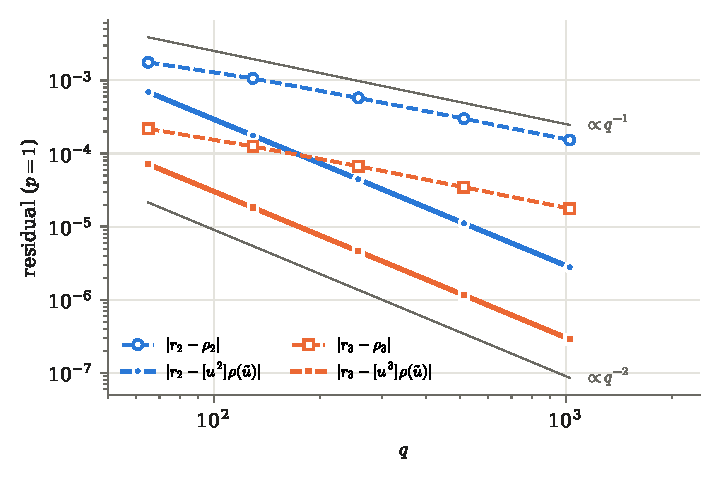
\includegraphics[width=0.78\textwidth]{figures/kinematic.pdf}
\caption{Residuals of the Taylor coefficients $r_2,r_3$ of $R_{1/q}$ against the renormalized family, with (solid) and without (dashed) the M\"obius substitution of Proposition~\ref{prop:kinematic}. The substitution removes the entire $O(1/q)$ part.}\label{fig:kinematic}
\end{figure}

Thus, through first order in $1/q$, the whole function $R_{p/q}$, and not only $\kappa$, is the renormalized family composed with the exact Inou--Shishikura phase. The renormalized germ itself has no $O(1/q)$ correction.

\section{The hierarchy and the constant $\kappa_*$}\label{sec:hierarchy}

\subsection{The iteration}
For $\alpha=[0;a_1,a_2,\ldots]$ the renormalization $\mathcal Rf_\alpha$ has multiplier $e^{-2\pi i/\alpha}$. Conjugating by $z\mapsto\bar z$ turns its rotation number into $1/\alpha\bmod1=[0;a_2,a_3,\ldots]$, so that $\mathcal R$ acts on continued fractions as the Gauss map~\cite{IS}. When the first $k$ partial quotients tend to infinity, each renormalization should therefore be close to $\mathcal P$ applied to the complex conjugate of the previous one. Write $\bar G(W)=\overline{G(\bar W)}$, normalize germs to the form $v+v^2+O(v^3)$, and set
\[
G_1=\PP,\qquad G_{k+1}=\mathcal P(\bar G_k),\qquad \kappa_k=\iota(G_k)-\tfrac12 .
\]
By Theorem~\ref{thm:horn-index}, $\kappa_k=a_2/(2\pi ia_1^2)$ for the horn map of $\bar G_{k-1}$. For $k\ge2$ the germs $G_k$ are given by convergent series of small radius (about $2.6$ in the normalized coordinate $v$ at $k=2$), and the horn maps must be sampled at heights where the orbits stay well inside the disc of convergence. Table~\ref{tab:levels} lists $\kappa_1,\ldots,\kappa_7$ for two independent settings of height, Fourier truncation and precision. They agree to $2\cdot10^{-14}$ or better at every level.

\begin{table}[t]
\centering\footnotesize
\begin{tabular}{@{}cllc@{}}
\toprule
$k$ & $\kappa_k$ ($h=1$) & $|\kappa_k-\kappa_{k-1}|$ & $|\kappa_k^{(h=1)}-\kappa_k^{(h=5/4)}|$ \\
\midrule
1 & $0.0238258874022 - 0.0523046591140\,i$ &  & --- \\
2 & $0.0112359215880 - 0.0377814219023\,i$ & $1.9\cdot10^{-2}$ & $6.1\cdot10^{-16}$ \\
3 & $0.0119510972606 - 0.0374792854625\,i$ & $7.8\cdot10^{-4}$ & $1.7\cdot10^{-14}$ \\
4 & $0.0119279615825 - 0.0374560782080\,i$ & $3.3\cdot10^{-5}$ & $5.8\cdot10^{-16}$ \\
5 & $0.0119292218902 - 0.0374555354669\,i$ & $1.4\cdot10^{-6}$ & $2.5\cdot10^{-17}$ \\
6 & $0.0119291812682 - 0.0374554947782\,i$ & $5.7\cdot10^{-8}$ & $9.9\cdot10^{-19}$ \\
7 & $0.0119291834806 - 0.0374554938253\,i$ & $2.4\cdot10^{-9}$ & $1.2\cdot10^{-19}$ \\
\midrule
$\infty$ & $0.011929183413 - 0.037455493752\,i$ & & \\
\bottomrule
\end{tabular}

\caption{The hierarchy $\kappa_k=\iota(G_k)-\frac12$, $G_{k+1}=\mathcal P(\bar G_k)$, computed at heights $h=1$ ($16$ Fourier modes, $90$ digits) and $h=\frac54$ ($14$ modes, $100$ digits). Level $1$ is $\kappa_0$ and is common to both. The last row is the extrapolation of Numerical result~\ref{obs:kstar}.}\label{tab:levels}
\end{table}

\begin{observation}\label{obs:kstar}
The differences $\Delta_k=\kappa_k-\kappa_{k-1}$ decrease geometrically: $|\Delta_{k+1}|/|\Delta_k|$ tends to $0.0419$, and the ratios are $\Delta_{k+1}/\Delta_k\approx-0.01546\mp0.03894\,i$, with imaginary parts of alternating sign (Figure~\ref{fig:hierarchy}). This is the signature of an antilinear contraction $\Delta\mapsto\nu\bar\Delta$, as expected since the linearization of $G\mapsto\mathcal P(\bar G)$ is antilinear. Fitting $\Delta_{k+1}=M\Delta_k$ with $M$ real-linear on $\C\cong\R^2$ gives eigenvalues $\pm0.041899$ and the limit
\[
\kappa_*:=\lim_{k\to\infty}\kappa_k=0.011929183413-0.037455493752\,i,
\]
with the fits through levels $6$ and $7$ differing by less than $2\cdot10^{-12}$. Thus $\kappa_*+\frac12=0.5119292-0.0374555\,i$ is the cubic coefficient of the normalized fixed point $G_*=\mathcal P(\bar G_*)$.
\end{observation}

\begin{figure}[t]
\centering
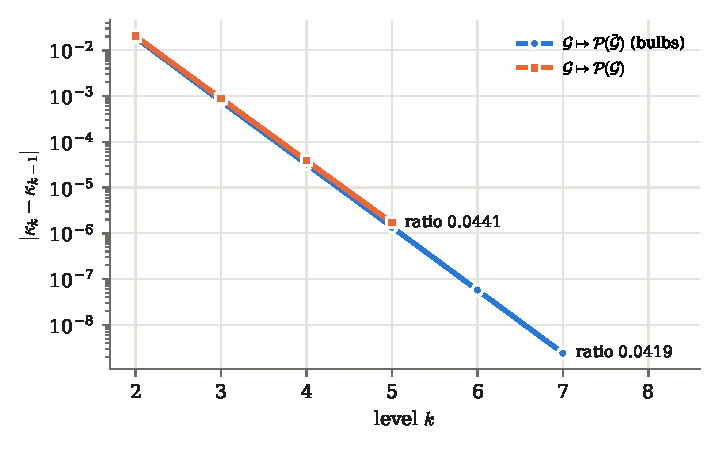
\includegraphics[width=0.78\textwidth]{figures/hierarchy.pdf}
\caption{Successive differences of the two hierarchies: $G\mapsto\mathcal P(\bar G)$, which governs the bulbs, and the holomorphic parabolic renormalization $G\mapsto\mathcal P(G)$ of Remark~\ref{rem:LY}. The labels give the last ratio of successive differences.}\label{fig:hierarchy}
\end{figure}

\begin{remark}[The holomorphic operator]\label{rem:LY}
Without the conjugation, $G\mapsto\mathcal P(G)$ is the parabolic renormalization operator whose fixed point $f_*$ was shown to exist by Inou and Shishikura and computed by Lanford and Yampolsky~\cite{LY}. They report $f_*(z)\approx z+z^2+(0.514-0.0346\,i)z^3$ and a leading eigenvalue $\approx-0.017+0.040\,i$ of $D\mathcal P$ at $f_*$. Our code without conjugation reproduces both: the cubic coefficients converge to $0.5142768-0.0346276\,i$ (extrapolated, $\pm10^{-7}$), and the ratio of successive differences tends to $-0.01764+0.04038\,i$. The bulbs, however, select the fixed point $G_*\ne f_*$ of the conjugated operator.
\end{remark}

\subsection{Comparison with bulbs}
\begin{conjecture}\label{conj:hierarchy}
For every $k\ge1$,
\[
\lim_{N_k\to\infty}\cdots\lim_{N_1\to\infty}\kappa\bigl([0;N_1,\ldots,N_k]\bigr)=\begin{cases}\kappa_k,&k\text{ odd},\\ \overline{\kappa_k},&k\text{ even}.\end{cases}
\]
In particular $\kappa_*$ and $\overline{\kappa_*}$ are the limits of the first correction as the number of large partial quotients of $p/q$ grows, along odd and even $k$ respectively.
\end{conjecture}

The case $k=1$ is Numerical result~\ref{obs:identity}. For $k=2$, formula \eqref{eq:boundedp} with $r=1$ gives the limit of $\kappa([0;N,p])$ as $N\to\infty$ as an index of $(e^{-2\pi i/p}\PP)^p$. We computed this index for $p\le256$ with the normal form of Theorem~\ref{thm:nf} generalized to arbitrary germs, an $O(p^3)$ recursion, and extrapolated in $1/p$. The result, $0.0112359330+0.0377814233\,i$, equals $\overline{\kappa_2}$ to $1.2\cdot10^{-8}$. The conjugate appears because $p^{-1}\bmod q\to0^-$ along this sequence, against $0^+$ for $p=1$. Without the conjugation in the definition of $G_2$ one obtains $0.014770-0.033911\,i$, which the data exclude.

We also tested the diagonal sequences $[0;N,\ldots,N]$, computing $\kappa$ with the normal form at $128$ and $192$ bits (the two agree to $4\cdot10^{-35}$) and fitting polynomials in $1/N$. For $k=2$ and $16\le N\le160$ ($q\le25601$) the limit agrees with $\overline{\kappa_2}$ to $3\cdot10^{-10}$, so the diagonal and the iterated limits coincide. For $k=3$ and $6\le N\le40$ ($q\le64080$) the limit is $0.0119509937-0.0374804294\,i$. It agrees with $\kappa_3$ to $1.2\cdot10^{-6}$, and every fit with $N\ge10$ and five or six terms lies within $1.4\cdot10^{-5}$ of $\kappa_3$. For comparison, $|\kappa_3-\kappa_2|=7.8\cdot10^{-4}$ and $|\kappa_3-\overline{\kappa_3}|=7.5\cdot10^{-2}$. Thus Conjecture~\ref{conj:hierarchy}, including its parity rule, holds numerically for $k\le3$. Level $4$, where $|\kappa_4-\kappa_3|=3.3\cdot10^{-5}$, would require periods $q\approx N^4$ with $N\gtrsim30$.

\section{Component dependence and the $\frac12$-root}\label{sec:component}

\subsection{The period-two disc}
Remark~\ref{rem:general} applies to the satellites of every hyperbolic component. For the period-two disc $W_{1/2}$, $c=-1+\lambda/4$, with $\lambda$ the multiplier of the attracting $2$-cycle, the values of $\kappa$ at generic $p/q$ are close to those of the cardioid at the same $p/q$~\cite{repo}, but the bounded-$p$ limits differ. The renormalization picture attributes these limits to the parabolic germ at the root of the component, here $c=-\frac34$. This point is also the root of the cardioid's own $\frac12$-satellite, which the cardioid approaches along $[0;1,1,m,\ldots]$ with $m\to\infty$. This suggests the following.

\begin{conjecture}[Root principle]\label{conj:root}
The limits of $\kappa$ and of $G$ along satellites $[0;N,t]$ of a hyperbolic component, as $N\to\infty$ with the tail $t$ fixed, depend only on the parabolic germ at the root of the component. In particular the satellite $[0;N,t]$ of $W_{1/2}$ and the satellite $[0;1,1,N-1,t]$ of the cardioid have the same limits.
\end{conjecture}

Table~\ref{tab:diskroot} confirms the second statement for three tails, and for the bulb size, to about $10^{-9}$. The disc values come from Cauchy integrals in the multiplier of the $2$-cycle, and the cardioid values from the normal form. When the first partial quotient stays bounded the correspondence fails: at $N=256$ the two sides differ by between $3\cdot10^{-5}$ and $1.5\cdot10^{-3}$ for the prefixes $(2,9,4)$, $(3,5)$, $(1,4)$, $(5,1,2)$ and $(7)$, and the disc is then closer to the cardioid at the same $p/q$. So only the first renormalization, and hence the germ at the root, distinguishes components.

\begin{table}[t]
\centering\footnotesize
\begin{tabular}{@{}lllc@{}}
\toprule
& disc $[0;N,\tau]$ & cardioid $[0;1,1,N-1,\tau]$ & $|\Delta|$ \\
\midrule
$\kappa$, $\tau=\varnothing$ & $0.01840526173 - 0.04290372357\,i$ & $0.01840526170 - 0.04290372213\,i$ & $1.4\cdot10^{-9}$ \\
$\kappa$, $\tau=2$ & $0.04755255860 - 0.01974956083\,i$ & $0.04755255811 - 0.01974956031\,i$ & $7.1\cdot10^{-10}$ \\
$\kappa$, $\tau=3$ & $0.05330701166 - 0.002605955494\,i$ & $0.05330701184 - 0.002605955354\,i$ & $2.2\cdot10^{-10}$ \\
$G$, $\tau=\varnothing$ & $1.020162587$ & $1.020162587$ & $5.3\cdot10^{-10}$ \\
\bottomrule
\end{tabular}

\caption{The period-two disc near its root against the cardioid near its $\frac12$-root. The disc column uses $[0;N,t]$ in the multiplier of the $2$-cycle, the cardioid column $[0;1,1,N-1,t]$. Both are extrapolated from $N=128,\dots,2048$ with three terms in $1/q$.}\label{tab:diskroot}
\end{table}

\subsection{The horn map of $-z+z^2$}
At $c=-\frac34$ the map is conjugate to $f(z)=-z+z^2$, and $g=f\circ f=z-2z^3+z^4$ has a triple fixed point at $0$. Its attracting petals lie along $\pm\R$ and its repelling petals along $\pm i\R$, and $f$ exchanges the members of each pair.

\begin{lemma}[Two-petal Fatou coordinate]\label{lem:fatou2}
There is a unique formal series
\[
\Phi(z)=\tfrac14z^{-2}+d_{-1}z^{-1}+\beta\log z+\sum_{k\ge1}d_kz^k
\]
with $\Phi\circ g=\Phi+1$. Its coefficients are rational: $d_{-1}=\frac14$, $\beta=\frac{11}8$, $d_1=-\frac5{16}$, $d_2=\frac{75}{64}$, $\ldots$ The coefficient $\beta$ is the r\'esidu it\'eratif $\frac32-\iota(g)$ of $g$, and $\iota(g)=\iota_{1/2}=\frac18$.
\end{lemma}

\begin{proof}
Write $g(z)=z(1+h)$ with $h=-2z^2+z^3$. Then $\Phi\circ g-\Phi=\sum_kd_kz^k\bigl((1+h)^k-1\bigr)+\beta\log(1+h)$, and $z^k((1+h)^k-1)=-2kz^{k+2}+O(z^{k+3})$. The coefficient of $z^m$ therefore contains $d_{m-2}$ with the factor $-2(m-2)$ for $m\ne2$, and $\beta$ with the factor $-2$ for $m=2$, together with unknowns of lower index. Solving order by order gives uniqueness, with the constant term $d_0$ free, and the stated values. The index is $\Res\,dz/(2z^3-z^4)=\frac18$, which agrees with $\iota_{1/2}$ in Remark~\ref{rem:exact}.
\end{proof}

Consider orbits leaving the repelling petal $+i\R$ above the height $\operatorname{Im}Z=\beta\pi/2\approx2.16$ in the Fatou coordinate. They reach the attracting petal $-\R$, and $f$, a half step of $g$, carries them to $+\R$. This defines an upper horn map $E_{1/2}(Z)=Z+a_0+\sum a_ne^{2\pi inZ}$ on the cylinder of $f$-orbits, and a parabolic germ $\Ph$ as in Section~\ref{sec:horn}.

\begin{observation}\label{obs:half}
Computed at the heights $4.5$ and $5.5$ with $100$ digits, which agree in all digits shown,
\begin{align*}
\operatorname{Re}\kappa_{1/2}&=\phantom{-}0.018405261617964781008961965439681,\\
\operatorname{Im}\kappa_{1/2}&=-0.042903723880230475207353337798906,
\end{align*}
where $\kappa_{1/2}:=\iota(\Ph)-\frac12$.
This agrees with the bulb limits of Table~\ref{tab:diskroot} to $3\cdot10^{-10}$ for the disc and $2\cdot10^{-9}$ for the cardioid. The germ $\Ph$ also carries the rest of the theory. With the phase $e^{-2\pi ir/p}$ and $r=1$ (since $[0;N,t]=t/(tN+1)$), formula \eqref{eq:boundedp} gives $0.04755255819-0.01974956104\,i$ for $t=2$ and $0.05330701191-0.00260595580\,i$ for $t=3$. The unfolding $e^{u}\Ph$ gives $G=1.0201625875$ for $p=1$ and $G=1.1070111364$ for $p=2$, against $1.107011147$ for disc bulbs along $2/(2N+1)$.
\end{observation}

The first-order coefficient of the disc, $\kappa_{W_{1/2}}(1/q)=\kappa_{1/2}+(-0.17743-0.19381\,i)/q+O(q^{-2})$, is not the kinematic value $-i/(2\pi q)$ of Corollary~\ref{cor:kinematic}. This is not a contradiction: at the degenerate parabolic point $c=-\frac34$ the multiplier of the $2$-cycle is not the Inou--Shishikura rotation, so Proposition~\ref{prop:kinematic} does not apply to it.

\section{Degree three: a second universality class}\label{sec:degree3}

For $z^3+c$ the main component is parametrized by the multiplier $\lambda$ of the fixed point $z=(\lambda/3)^{1/2}$, with $c=z-z^3$. Its cusp at $\lambda=1$, where $z_*=1/\sqrt3$ and $c_*=2/(3\sqrt3)$, has the parabolic germ $w\mapsto w+\sqrt3\,w^2+w^3$. In $v=\sqrt3\,w$ this is
\[
g(v)=v+v^2+\tfrac13v^3,
\]
whose r\'esidu it\'eratif is $1-\frac13=\frac23$. Lemma~\ref{lem:fatou} generalizes with $F(w)=-1/g(-1/w)$ and $\Phi(w)=w-\frac23\log w+\sum c_kw^{-k}$, where $c_1,c_2,\ldots=\frac29,\frac5{54},\frac{14}{243},\frac{89}{2430},\ldots$. The horn map gives, at 50 and at 70 digits,
\[
\kappa_0^{(3)}:=\frac{a_2}{2\pi ia_1^2}=0.143599278095291569488064104088-0.030311647898502537611943110858\,i .
\]
Table~\ref{tab:deg3} shows that $\kappa_3(1/q)+\frac i{2\pi q}$ converges to this value like $q^{-2}$. The correction $-i/(2\pi q)$ is thus the same as in degree two, as Corollary~\ref{cor:kinematic} predicts, while the constant is not. The bounded-$p$ predictions hold in degree three as well: $\kappa$ agrees to within $5\cdot10^{-6}$ for $(p,r)=(1,1),(2,1),(3,1),(3,2)$ at $q\approx512p$.

\begin{table}[t]
\centering\small
\begin{tabular}{@{}rll@{}}
\toprule
$q$ & $\kappa_3(1/q)$ & $|\kappa_3(1/q)+\tfrac{i}{2\pi q}-\kappa_0^{(3)}|$ \\
\midrule
128 & $0.1436180525 - 0.03147252376\,i$ & $8.5\cdot10^{-5}$ \\
256 & $0.1436043106 - 0.03091278634\,i$ & $2.1\cdot10^{-5}$ \\
512 & $0.1436005784 - 0.03061736682\,i$ & $5.3\cdot10^{-6}$ \\
1024 & $0.1435996091 - 0.03046578964\,i$ & $1.3\cdot10^{-6}$ \\
\midrule
horn map of $v+v^2+\tfrac13v^3$ & $0.1435992781 - 0.03031164790\,i$ & \\
\bottomrule
\end{tabular}

\caption{Degree three: $\kappa_3(1/q)$ from Cauchy integrals on $|u|=1$ (Appendix~\ref{app:num}) against the horn map of the cubic cusp germ.}\label{tab:deg3}
\end{table}

The bulb size needs one more observation.

\begin{proposition}\label{prop:antipodes}
Let $W$ be a bounded hyperbolic component of $z^d+c$. Its multiplier map $\rho:W\to\D$ has the form $\rho=\phi^{\,d-1}$ with $\phi:W\to\D$ a conformal isomorphism. In particular $\rho=-1$ at exactly $d-1$ points of $\partial W$.
\end{proposition}

\begin{proof}
The map $\rho$ is proper, since the cycle becomes indifferent at $\partial W$. Its zeros are the parameters at which the critical point lies on the cycle; there is exactly one, the centre, because $W$ is a cell with a unique centre~\cite{MilnorHC}. At the centre $c_0$ we have $\rho=\prod_jd\,z_j^{d-1}$ with one factor $z_j=f_c^n(0)$ vanishing. Moreover $c_0$ is a simple zero of $P(c)=f_c^n(0)$: $P$ has integer coefficients and $P'\equiv1\pmod d$ by induction, so $P'(c_0)\ne0$ at the algebraic integer $c_0$ (Gleason's argument). Hence $\rho$ vanishes to order exactly $d-1$ at $c_0$. A proper holomorphic map from a disc to $\D$ with a single zero of order $d-1$ is a Blaschke product $\phi^{d-1}$ with $\phi$ a conformal isomorphism.
\end{proof}

In degree three, then, there are two points with multiplier $-1$, and both are predicted. At $p=3$, $r=1$, the horn map gives $G=1.196074$ and $1.227092$, against the extrapolated bulb values $1.196075$ and $1.227091$.

\section{Arithmetic nature}\label{sec:pslq}

For each of $\kappa_0$, $\kappa_0^{(3)}$ and $\kappa_{1/2}$ we searched with PSLQ~\cite{PSLQ}, at $28$ digits and coefficient bound $1000$, for integer relations between the real part, the imaginary part, the squared modulus or the argument divided by $\pi$, and every subset of at most three of $\{1,\pi,\pi^2,1/\pi,\log2,\zeta(3),G,\gamma\}$, where $G$ is Catalan's constant. For $\kappa_0$ we also tried $\operatorname{Re}(2\pi i\kappa_0)$, $\operatorname{Im}(2\pi i\kappa_0)$, $|a_1|$ and $\arg a_1/\pi$. No relation was found. This is consistent with the general expectation that invariants of parabolic germs, such as the \'Ecalle--Voronin moduli~\cite{Ecalle,Voronin}, are transcendental numbers without closed form. We regard $\kappa_0$, $\kappa_0^{(3)}$ and $\kappa_{1/2}$ as new constants of this kind.

\section{Discussion}\label{sec:discussion}

The first-order theory of the satellite bulbs is the Ford-circle picture, with radii $q^{-2}$ and Farey tangencies. The first correction, $\kappa(p/q)$, is the holomorphic index of a parabolic germ (Theorem~\ref{thm:index}), and it equals the index of the rotation quotient minus $\frac12$ (Corollary~\ref{cor:quotient}). Numerically it is controlled by near-parabolic renormalization. The constant $\kappa_0$ comes from the simplest instance, $\alpha=1/q\to0$. Bounded $p$ corresponds to one renormalization step with phase $e^{-2\pi ir/p}$, and the first order in $1/q$ comes from the exact M\"obius phase. Large partial quotients correspond to iterated renormalization, which contracts by a factor $0.042$ per step towards a fixed point that differs from the classical one. Hyperbolicity of $\mathcal R$ would explain why $\kappa(p/q)$ depends mainly on the last partial quotients, that is, on $p^{-1}\bmod q$~\cite{repo}. Finally, the component enters only through the germ at its root. Farey-type combinatorics survives at every order, but the metric data at a rational are those of a parabolic germ, and they are transcendental.

\subsection*{Open problems}
\begin{enumerate}
\item Prove Conjecture~\ref{conj:main}, for instance by establishing a conformal conjugacy between $\Phi_{1/q}$ and $\mathcal Rf_{1/q}$ together with continuity of $\mathcal R$ at integer $1/\alpha$.
\item Prove Conjecture~\ref{conj:unfolding}, in particular that the renormalized germ has no $O(1/q)$ correction beyond the phase of Proposition~\ref{prop:kinematic}. By Corollary~\ref{cor:kinematic} this gives the universal term $-i/(2\pi pq)$. Identify the $O(q^{-2})$ term.
\item Prove Conjecture~\ref{conj:hierarchy}, and describe the fixed point $G_*$ of $G\mapsto\mathcal P(\bar G)$ and its spectrum.
\item Compute the generic limit function $\kappa(p/q)$, $p\to\infty$, by iterated renormalization with bounded partial quotients, including its values at quadratic irrationals as periodic points of $\mathcal R$.
\item Prove Conjecture~\ref{conj:root}. Derive the first-order coefficient $-0.17743-0.19381\,i$ of the disc from the kinematics of the degenerate parabolic point $c=-\frac34$, and treat the roots of other components in the same way.
\item Decide whether $\kappa_0$ can be expressed in closed form through the \'Ecalle--Voronin invariants of $z+z^2$.
\end{enumerate}

\appendix
\section{Numerical methods and error control}\label{app:num}

\subsection*{A.1 Normal form}
Recursion \eqref{eq:rec} was run in \texttt{mpmath}~\cite{mpmath} at $50$ working digits for $64\le q\le8192$ ($p=1$) and $q\le8193$ (bounded $p$). It was also implemented in Arb ball arithmetic~\cite{Arb}. There the online convolution $(H^2)_k$ is evaluated in blocks: completed blocks are folded in by truncated series products, and the remainder is summed directly. The working precision is doubled until the certified radius of $\kappa$ is below $10^{-40}$. For $p=1$ the radii are $1.6\cdot10^{-50}$ at $q=1024$ and below $2\cdot10^{-111}$ at $q=32768$, and the two implementations agree to the $40$ digits stored. The ball version is $60$--$110$ times faster; $q=32768$ takes about two minutes. For generic $p$ the coefficients $H_k$ are very large and ball radii, which cannot see cancellation, grow until they carry no information. For those values we ran the same code in midpoint arithmetic at two precisions, $128$ and $192$ bits, and took their difference as the error; it never exceeded $4\cdot10^{-35}$. The recursion for general germs used in Section~\ref{sec:hierarchy} was run in \texttt{mpmath} at $40$--$60$ digits.

\subsection*{A.2 Extrapolation}
Limits in $q$ or $N$ come from least-squares fits in powers of $1/q$ or $1/N$, solved by QR decomposition at $40$--$80$ digits. Each is reported only when it is stable, to the stated precision, under changes of the fit order and of the smallest $q$ used. The limit of the hierarchy (Numerical result~\ref{obs:kstar}) uses a real-linear model $\Delta_{k+1}=M\Delta_k$ fitted to the last three differences. This model is exact for both linear and antilinear geometric contractions, whereas componentwise Aitken extrapolation is not exact for antilinear ones.

\subsection*{A.3 Horn maps}
For the cusp germs the Fatou series were truncated at $K=40$ terms and evaluated at $|w|\ge800$, where the truncation error is below $10^{-60}$; the coefficients $|c_k|$ grow roughly like $k!/(2\pi)^k$. We used $n=1000$--$1800$ repelling iterations and computed Fourier coefficients from $64$--$80$ samples on $\operatorname{Im}Z=\frac14$, with aliasing below $10^{-58}$. For the germs $G_k$ of the hierarchy, which are known only as convergent series, the horn maps were sampled at $\operatorname{Im}Z=1$ and $\frac54$ so that all orbits stay well inside the disc of convergence. A first run at $\operatorname{Im}Z=\frac12$ was inaccurate at the $10^{-3}$ level and was discarded. For the two-petal germ of Section~\ref{sec:component} the exact series of Lemma~\ref{lem:fatou2} was truncated at $K=40$--$60$, with $900$--$1000$ iterations of $g$ and samples at $\operatorname{Im}Z=4.5$--$5.5$, well above the centre $\beta\pi/2$ of the repelling cylinder. A Fourier coefficient $a_n$ extracted at height $h$ carries noise amplified by $e^{2\pi nh}$, and the working precision ($60$--$160$ digits) was chosen accordingly. Independent heights agree to all digits reported.

\subsection*{A.4 Multiplier data}
The Taylor coefficients $r_k$ were computed by Cauchy integrals of $R_{p/q}$ over a circle, continuing the $q$-cycle numerically, and those of the renormalized families in the same way. For $z^2+c$ radii up to $|u|=2.5$ are admissible. For $z^3+c$ the function $R_{p/q}$ has a singularity inside $|u|<2.5$, and the radius must be at most $1.5$. The condition $r_1=-1$ of Theorem~\ref{thm:index} is a reliable diagnostic: on the larger circle it fails, with $r_1=-1.032$. In degree three each satellite has two antipodes (Proposition~\ref{prop:antipodes}), and both were continued in the target multiplier from $0$ to $-1$.

\subsection*{A.5 Reproducibility}
All code, data and tests are in the accompanying repository~\cite{repo}. The package \texttt{bulbford} contains the normal forms (\texttt{normal\_form}, \texttt{normal\_form\_ball}), the horn maps (\texttt{horn}, \texttt{horn\_half}), the germ and renormalization tools (\texttt{germ}, \texttt{renorm}), the extrapolation (\texttt{extrapolate}) and the dynamics (\texttt{dynamics}, whose cycle iteration is compiled with Numba). Every table and figure is generated from the data files by \texttt{paper/tables.py} and \texttt{paper/figures.py}. The test suite checks Theorems~\ref{thm:index} and~\ref{thm:nf}, the value of $\kappa_0$ to $25$ digits, the bounded-$p$, kinematic, hierarchy and degree-three predictions, and the constant $\kappa_{1/2}$.

\subsection*{Data availability}
All data supporting the results are contained in the repository~\cite{repo}.

\subsection*{Acknowledgments}
The computations and the drafting of this paper were carried out with the assistance of an AI system (Claude, Anthropic).

\begin{thebibliography}{99}
\bibitem{BE} X.~Buff and A.~Epstein, \emph{A parabolic Pommerenke--Levin--Yoccoz inequality}, Fund. Math. \textbf{172} (2002), 249--289.
\bibitem{DH} A.~Douady and J.~H.~Hubbard, \emph{\'Etude dynamique des polyn\^omes complexes}, Parties I et II, Publications Math\'ematiques d'Orsay 84-02 and 85-04, 1984--1985.
\bibitem{Ecalle} J.~\'Ecalle, \emph{Les fonctions r\'esurgentes}, Tomes I--III, Publications Math\'ematiques d'Orsay, 1981--1985.
\bibitem{PSLQ} H.~R.~P.~Ferguson, D.~H.~Bailey and S.~Arno, \emph{Analysis of PSLQ, an integer relation finding algorithm}, Math. Comp. \textbf{68} (1999), 351--369.
\bibitem{FM} A.~C.~Fowler and M.~J.~McGuinness, \emph{The size of Mandelbrot bulbs}, Chaos Solitons Fractals X \textbf{3} (2019), 100019.
\bibitem{Ford} L.~R.~Ford, \emph{Fractions}, Amer. Math. Monthly \textbf{45} (1938), 586--601.
\bibitem{GM} J.~Guckenheimer and R.~McGehee, \emph{A proof of the Mandelbrot $N^2$ conjecture}, Report No.~15, Institut Mittag-Leffler, 1984.
\bibitem{IS} H.~Inou and M.~Shishikura, \emph{The renormalization for parabolic fixed points and their perturbation}, preprint; see \url{https://www.math.kyoto-u.ac.jp/~mitsu/pararenorm/}.
\bibitem{Arb} F.~Johansson, \emph{Arb: efficient arbitrary-precision midpoint-radius interval arithmetic}, IEEE Trans. Comput. \textbf{66} (2017), 1281--1292.
\bibitem{LY} O.~E.~Lanford III and M.~Yampolsky, \emph{Fixed Point of the Parabolic Renormalization Operator}, SpringerBriefs in Mathematics, Springer, 2014; arXiv:1108.2801.
\bibitem{Lavaurs} P.~Lavaurs, \emph{Syst\`emes dynamiques holomorphes: explosion de points p\'eriodiques paraboliques}, Th\`ese, Universit\'e Paris-Sud, Orsay, 1989.
\bibitem{Milnor} J.~Milnor, \emph{Dynamics in One Complex Variable}, 3rd ed., Annals of Mathematics Studies 160, Princeton University Press, 2006.
\bibitem{MilnorHC} J.~Milnor, \emph{Hyperbolic components} (with an appendix by A.~Poirier), in: Conformal Dynamics and Hyperbolic Geometry, Contemp. Math. \textbf{573}, Amer. Math. Soc., 2012, 183--232.
\bibitem{mpmath} The mpmath development team, \emph{mpmath: a Python library for arbitrary-precision floating-point arithmetic}, \url{https://mpmath.org}.
\bibitem{repo} \emph{mandelbrot-bulbs-and-ford-circles-research}, code and data repository accompanying this paper, including the research register \texttt{RESEARCH\_bulb-ford-correction.md}.
\bibitem{Sh} M.~Shishikura, \emph{Bifurcation of parabolic fixed points}, in: The Mandelbrot Set, Theme and Variations (Tan Lei, ed.), London Math. Soc. Lecture Note Ser. 274, Cambridge Univ. Press, 2000, 325--363.
\bibitem{Voronin} S.~M.~Voronin, \emph{Analytic classification of germs of conformal mappings $(\C,0)\to(\C,0)$ with identity linear part}, Funct. Anal. Appl. \textbf{15} (1981), 1--13.
\end{thebibliography}

\end{document}
